\documentclass{beamer}
%\usetheme{Boadilla}
\usetheme{Darmstadt}

\title{Multi-Agent Learning - TFE Proposal}
%\subtitle{Using Beamer}
\author{Koen Boeckx}
\institute{RMA}
\date{\today}

\begin{document}

\begin{frame}
\titlepage
\end{frame}

\begin{frame}
\frametitle{Overview}
\begin{itemize}
    \item What is Multi-Agent (MA) learning
    \item What is Reinforcement Learning (RL)?
    \item How do we combine both?
    \item What am I working on?
    \item Where can you work on?
\end{itemize}
\end{frame}

\begin{frame}
\frametitle{What is Multi-Agent (MA) learning?}
\begin{itemize}
    \item Multiple `agents` act in an environment.
    \item The `environment` has rules
        \begin{itemize}
            \item Which actions are allowed?
            \item What are the consequences of actions?
        \end{itemize} 
    \item How does the opponent behave?
    \item How can agents coordinate actions to achieve optimal result?
\end{itemize}
\end{frame}

\begin{frame}
\frametitle{What is Reinforcement Learning (RL)?}
\begin{itemize}
    \item What is Machine Learning?
        \begin{itemize}
            \item \emph{Supervised Learning}: Learn from examples $(\mathbf{x}, y) \rightarrow y = f(\mathbf{x})$
            %\item $(\mathbf{x}, y) \rightarrow y = f(\mathbf{x})$
            \item Example: detect cats in Youtube videos
        \end{itemize}
    \item If we don't have the result $y$, but only a reward signal $r$?
    \begin{itemize}
        \item \emph{Reinforcement Learning}
        \item The agent learns a behavior through interaction with his environment
        \item Learning is done with neural networks
        \item Example: Control of a robot arm
    \end{itemize}
\end{itemize}
\begin{figure}[htp]
    \centering
    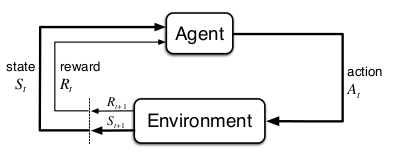
\includegraphics[width=8cm]{images/mdp.png}
    %\caption{The agent-environment interface of an MDP (reproduced from \cite{sutton2018reinforcement})}
    \label{fig:mdp}
\end{figure}
\end{frame}

\begin{frame}
\frametitle{How do we combine both? Multi-Agent RL}
\begin{itemize}
    \item Multiple agents interact with the environment and each other
    \item They (try to) learn a how to act:
        \begin{itemize}
            \item How to coordinate actions to achieve common goal?
            \item How to compete with other players for resources?
        \end{itemize}
    \item Every agent / team receives a reward to steer learning
    \item Problem is difficult because non-stationary environment
    \item Example: AlphaGo
\end{itemize}
\end{frame}

\begin{frame}
\frametitle{What am I working on?}
\begin{itemize}
    \item Can we use MARL to develop tactics and procedures in real circumstances?
    \item Multiple tanks have to learn how to coordinate their movements and fire to beat opponent(s)
    \item To do this, we:
        \begin{itemize}
            \item Develop a simplified model of a battlefield
            \item Simulate the actions a tank can take
            \item The agents (tanks) learn themselves how to move and which enemies to engage
        \end{itemize}
\end{itemize}
\end{frame}

\begin{frame}
    \begin{figure}
    \centering
    \begin{minipage}{.5\textwidth}
      \centering
      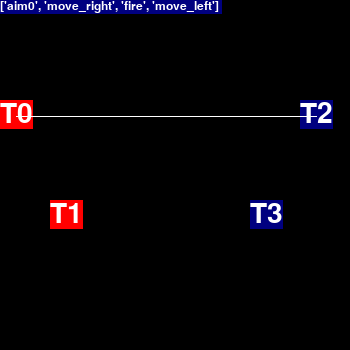
\includegraphics[width=4cm]{images/animation01/screenshot0-1.png}
    \end{minipage}%
    \begin{minipage}{.5\textwidth}
      \centering
      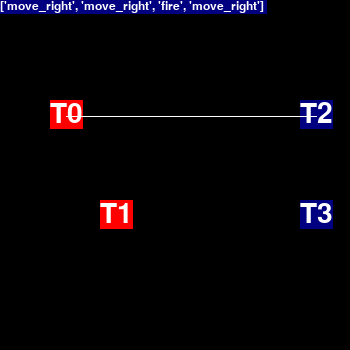
\includegraphics[width=4cm]{images/animation01/screenshot0-2.png}
    \end{minipage}
    %\end{figure}
    %\begin{figure}
    \centering
    \begin{minipage}{.5\textwidth}
      \centering
      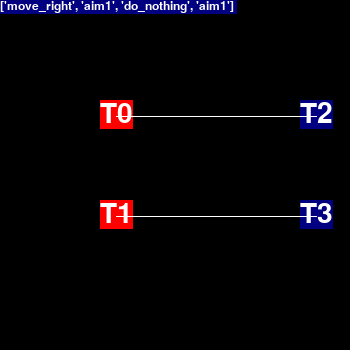
\includegraphics[width=4cm]{images/animation01/screenshot0-3.png}
    \end{minipage}%
    \begin{minipage}{.5\textwidth}
      \centering
      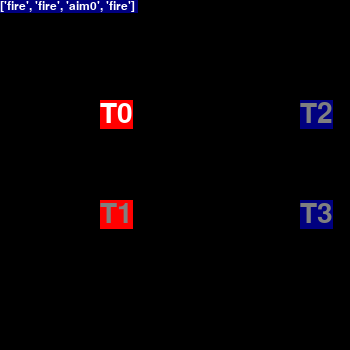
\includegraphics[width=4cm]{images/animation01/screenshot0-4.png}
    \end{minipage}
%    \caption{A simple learned tactic}
    \label{fig:simple_tactic01}
    \end{figure}
\end{frame}

\begin{frame}
\frametitle{Research questions}
\begin{itemize}
   \item Reward shaping: what is the reward we offer to a player / team?
    \item How complex should the neural network be?
    \item Communication between agents during learning and/or execution
    \item Is what we learned still valid when the terrain changes?
    \item Can we improve performance for real-time processing?
\end{itemize}
\end{frame}

\begin{frame}
\frametitle{What will you learn?}
\begin{itemize}
    \item Lots of programming (Python)
    \item Deep learning: how to train complex neural networks
    \begin{itemize}
        \item {\tt PyTorch}, {\tt TensorFlow}, ...
    \end{itemize}
    \item Interesting problem
        \begin{itemize}
            \item Many interacting subsystems
            \item Lots of room for improvement / creativity / own ideas
        \end{itemize} 
\end{itemize}
\end{frame}

\begin{frame}%[plain,c]
%\frametitle{A first slide}

\begin{center}
\Huge Any questions?
\end{center}

\end{frame}

\end{document}